\documentclass[11pt]{article}
\usepackage{icmlko}
\begin{document}

\title{부풀림을 빼도 안 된다 --- 문제는 수준이 아니라 그 행에 신호가 없다는 것}
\author{월드모델 실험실}
\date{노트 360 · 2026년 8월 1일}
\maketitle

\begin{abstract}
노트 359가 문 하나를 가리켰다 --- 팝업 전용 축은 학습 65행이 있어야
짝 규약에서 살고, 주최자 주장 라벨을 \emph{기준 안에서 중심 맞춰 학습에만}
넣으면 $24 \to 141$ 이 된다. 했다. \textbf{둘 다 답이 나왔고 하나는
내 예측을 뒤집었다.}

\textbf{하나 --- 노트 359의 계산이 맞았다.} 전용 축 넷이 주는 값이 학습
24행에서 $+0.0004$(2/12)였는데 141행에서 $+0.0056$(\textbf{8/12})이다.
부트스트랩 두 번($0.63^2$)이 문턱을 정한다는 셈이 관측과 맞는다.

\textbf{둘 --- 정규화는 실패했고, 그래서 노트 357의 설명이 반쪽이었다.}
미리 적었다: ``부풀림이 원인이라면 정규화한 E 는 0 이상이어야 한다.
0 아래면 노트 357의 기제 설명이 틀린 것이다.'' 결과는 팝업
$\mathbf{-0.0706}$(SD 0.0345, \textbf{0/12}) --- 정규화 안 한 노트 357의
$-0.0391$ 보다 \emph{더} 나쁘다. \textbf{곱셈 부풀림은 유보에서 순위를
섞는 문제를 설명하지만 학습에서 해로운 이유는 아니다.} 그 이유는 노트
357이 이미 잰 다른 수에 있다 --- 주장 행은 2025년에 $\rho = +0.0070$ 으로
\emph{축과 라벨 사이에 관계가 없다.} 신호 없는 행 117개를 학습에 넣으면
있는 신호가 묽어진다.

안 넣는다. 그리고 팝업 줄기가 닫힌다 --- \textbf{팝업에 필요한 것은 아무
행이 아니라 \emph{센} 행이다.}
\end{abstract}

\section{두 팔}

채점 집합을 건드리지 않았다 --- 세 팔 모두 유보 65행 · 판 분모 2,723 이다.
바뀌는 것은 학습뿐이라 과제가 그대로다(노트 224의 규약이 막는 것은 라벨을
다시 정의해 \emph{점수}를 바꾸는 일이다). 중심값은 학습 행으로만 쟀다.

\begin{center}
\begin{tabular}{llrr}
\hline
팔 & 팝업 & 학습 & 살아있는 열 \\
\hline
A 현행                     & 89행  & 24  & 5 \\
E 주장 정규화해 학습에      & 206행 & 141 & 5 \\
F E $+$ 전용 축 넷         & 206행 & 141 & \textbf{9} \\
\hline
\end{tabular}
\end{center}

\begin{center}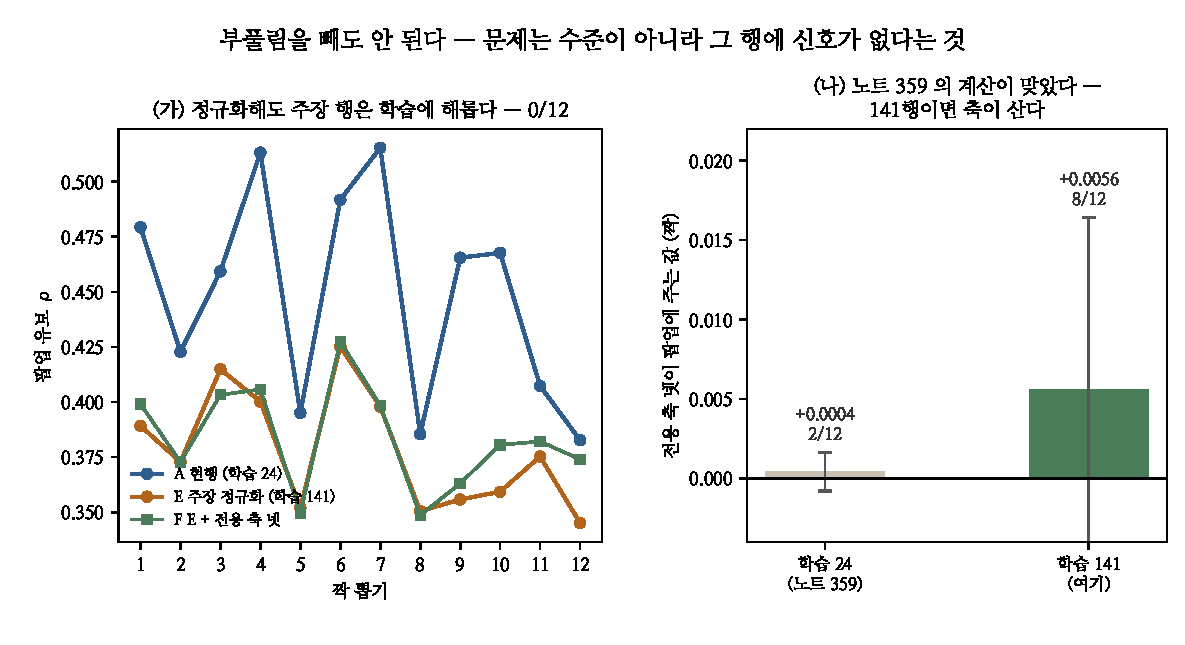
\includegraphics[width=\linewidth]{figs/norm.pdf}\end{center}

\section{노트 359의 계산이 맞았다}

\begin{center}
\begin{tabular}{lrrr}
\hline
전용 축 넷이 팝업에 주는 값 & 차 & SD & 부호 \\
\hline
학습 24행 (노트 359) & $+0.0004$ & 0.0012 & 2/12 \\
학습 141행 (여기)    & $\mathbf{+0.0056}$ & 0.0108 & \textbf{8/12} \\
\hline
\end{tabular}
\end{center}

노트 359가 셈으로 예측한 자리다 --- 자루 안 유효 행이 24행에서 9.8,
141행에서 56 이고 잎 최소가 20 이다. \textbf{예측한 대로 문턱을 넘으니
살아난다.} 노트 281의 법칙을 짝 규약으로 옮긴 것이 맞았다는 확인이고,
이번 창에서 미리 적은 셈이 관측을 맞힌 두 번째다(첫 번째는 노트 351의
환율).

\section{정규화는 실패했다 --- 그리고 내 예측이 뒤집혔다}

\begin{center}
\begin{tabular}{lrrr}
\hline
 & 판 & 팝업 & 팝업 부호 \\
\hline
E $-$ A & $-0.0019$ (4/12) & $\mathbf{-0.0706}$ (SD 0.0345) & \textbf{0/12} \\
F $-$ A & $-0.0014$ (4/12) & $-0.0651$ (SD 0.0342) & 0/12 \\
\hline
\end{tabular}
\end{center}

미리 적어 둔 것을 그대로 옮긴다.

\begin{quote}
E$-$A: 노트 357의 미정규화 판이 팝업 $-0.0391$ 이었다. 정규화가 그 손해의
원인이라면 E 는 0 이상이어야 한다. \textbf{0 아래면 부풀림이 원인이
아니었다는 뜻이고 그때 노트 357의 기제 설명이 틀린 것이다.}
\end{quote}

$-0.0706$ 에 0/12 다. \textbf{정규화한 쪽이 안 한 쪽보다 더 나쁘다.}

\textbf{그래서 노트 357을 정정한다.} 그 글이 잰 것 --- 주장 라벨이 해마다
$+0.27 \cdot +0.44 \cdot +0.20$ 부풀어 있고, 그래서 유보에서 섞으면
스피어만이 크기가 아니라 기준으로 줄을 선다 --- 은 맞다. \textbf{틀린 것은
그 기제를 \emph{학습} 손해에도 갖다 붙인 것이다.} 학습에서는 수준이
문제가 아니다. F18 은 도메인 안에서 라벨을 순위로 바꿔 쓰므로 중심을
빼든 안 빼든 학습 목표가 거의 같다 --- 실제로 두 판의 차가 $-0.0391$ 대
$-0.0706$ 으로 \emph{같은 쪽}이다.

\textbf{진짜 이유는 같은 글의 다른 수에 있었다.} 주장 행은 2025년에
$\rho = +0.0070$(n=37)이다 --- 축과 라벨 사이에 관계가 없다. 117행을
넣으면 24행이 갖고 있던 관계가 묽어진다. \textbf{학습에서 해로운 것은
부풀림이 아니라 무신호다.}

\section{팝업 줄기를 닫는다}

노트 352가 대표 수치의 구간을 $[0.257,\,0.660]$ 으로 잰 뒤 노트
357$\cdot$358$\cdot$359$\cdot$360 이 네 편에 걸쳐 그것을 좁히려 했다.

\begin{center}
\begin{tabular}{ll}
\hline
시도 & 결과 \\
\hline
계수 필터 풀기(유보까지) & 팝업 $0.49 \to 0.28$ --- 기준이 안 섞인다(357) \\
등급 필터 풀기           & \textbf{넣었다} --- 팝업 $+0.0140$(9/12), 유보 $59\to65$(358) \\
전용 축 되살리기         & 학습 24 로는 자루가 문턱을 못 넘는다(359) \\
주장 정규화해 학습에      & 팝업 $-0.0706$(0/12) --- 무신호 행이다(360) \\
\hline
\end{tabular}
\end{center}

\textbf{남은 결론 하나: 팝업에 필요한 것은 아무 행이 아니라 \emph{센}
행이다.} 실측(입장 · 참여 계수) 이력을 더 모으는 것 말고는 길이 없고,
그것은 수집이지 분석이 아니다. 지금 실측 학습이 24행이고 전용 축이 살려면
65행이 필요하다 --- \textbf{41행을 더 세어야 한다.}

\section{규약에 더하는 줄}

\begin{itemize}
\item \textbf{한 기제로 두 실패를 설명하려 하지 마라.} 노트 357의 부풀림은
유보 섞임을 설명하고 학습 손해는 설명하지 못한다. 두 실패는 같은 자료의
다른 성질에서 온다.
\item \textbf{학습에 행을 더할 때는 그 행들의 축$\to$라벨 관계를 먼저
잰다.} 주장 행의 2025년 $\rho$ 가 $+0.0070$ 이라는 것은 노트 357에 이미
적혀 있었다 --- 읽고 안 썼다.
\item \textbf{미리 적은 조건이 뒤집히면 그 자리에서 기제를 정정한다.}
이번 창에서 세 번 있었다(353 · 358 · 360).
\end{itemize}

\section{남은 것}

\begin{center}
\begin{tabular}{ll}
\hline
갈래 & 지금 아는 것 \\
\hline
팝업 실측 41행 & 수집. 그러면 전용 축이 산다 \\
만화 2026 스무 건 & 노트 356. 열한 번째 채점 도메인 \\
만화가 왜 누르나 & 노트 356. 라벨 종류로는 안 갈린다 \\
잎 문턱을 도메인별로 & 노트 359. 노트 259의 ``복도'' 문제가 걸린다 \\
\hline
\end{tabular}
\end{center}

\end{document}
